\subsection{Player}
\begin{wrapfigure}{L}{0.55\linewidth}
	\vspace{-10px}
	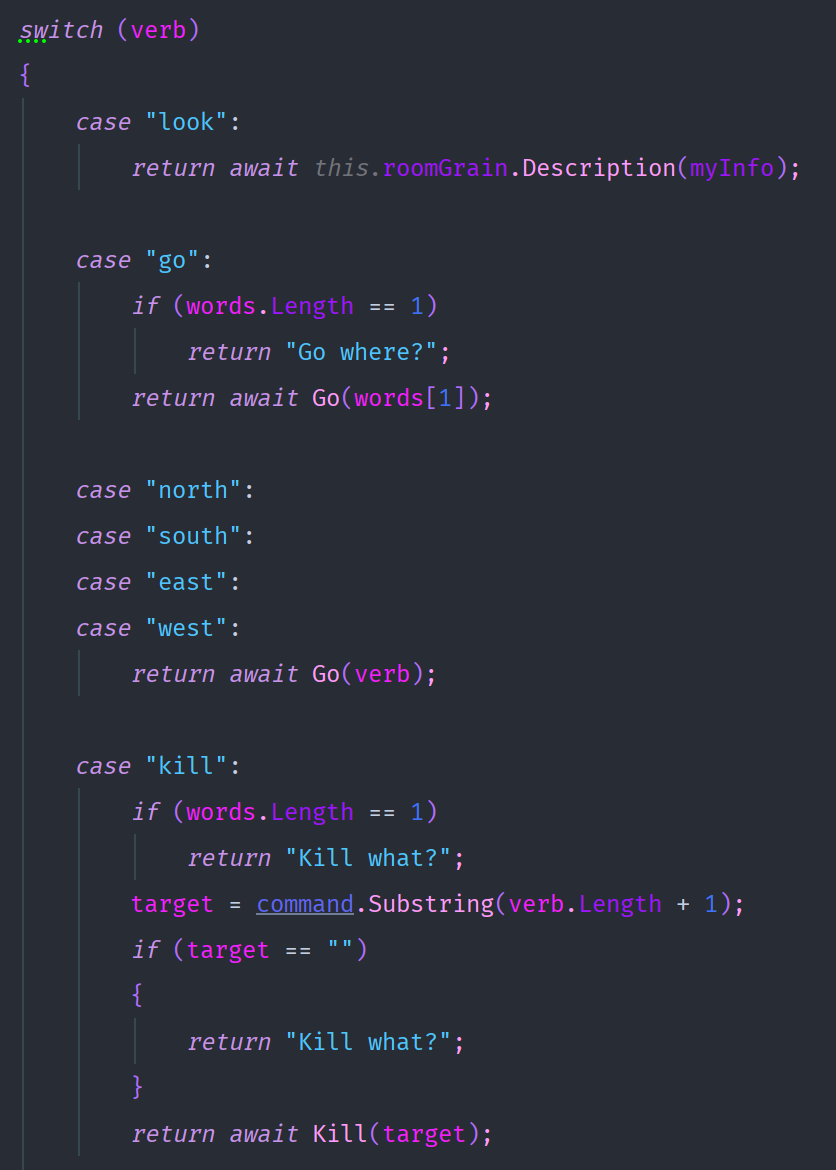
\includegraphics[width=\linewidth]{Materials/Decomposition/switchcases}
	\caption{Part of the switch case in player showing how some actions are implemented.}
\end{wrapfigure}
The player was the first object we implemented and the first we combinated. To understand how we chose to decompose the player we will first look at what makes a player. The player is implemented with a switch case with a case for all the actions the player can take. If we want to move to a new room we could for instance use the command 'go' followed by the direction we want to move. We can semantically look at the switch case as our 'case' or 'cases'.\\
A big part of what makes a player is the abilities it can use. For our implementation we have three variations of what abilities a player can use: fireball, roar or none. As already mentioned \todo{Reference our implementation} does the fireball and roar fulfil two different purposes. The fireball deals damage, and the roar makes the player take less damage. This left us with a choice of either accepting that we would need more information in the form of an extra combinator to ensure that we do not end up with dead code, or to accept the dead code, but making modularization  easier.\\
In our first iteration of the player we wanted to avoid the dead code. This made it hard to modularize the concept of an ability. The fireball simply calls the enemy's take damage function with a higher damage value than the player's standard attack. On the other hand, the roar ability sets a flag in the player which ensures when an enemy attacks, another branch is taken in the player's \textit{TakeDamage} method. The method can be seen in \autoref{PlayerTakeDamage}. To avoid dead code we added more semantic information when we created our repository. Two combinators which provided code with semantic type \textit{'damageTaken'} were thus made. The first having an implementation which did not use the field \textit{'roarActive'} and only had a single line for taking damage, and the second having the full if statement as seen in \autoref{PlayerTakeDamage}.

\begin{figure}[H]
	\centering
	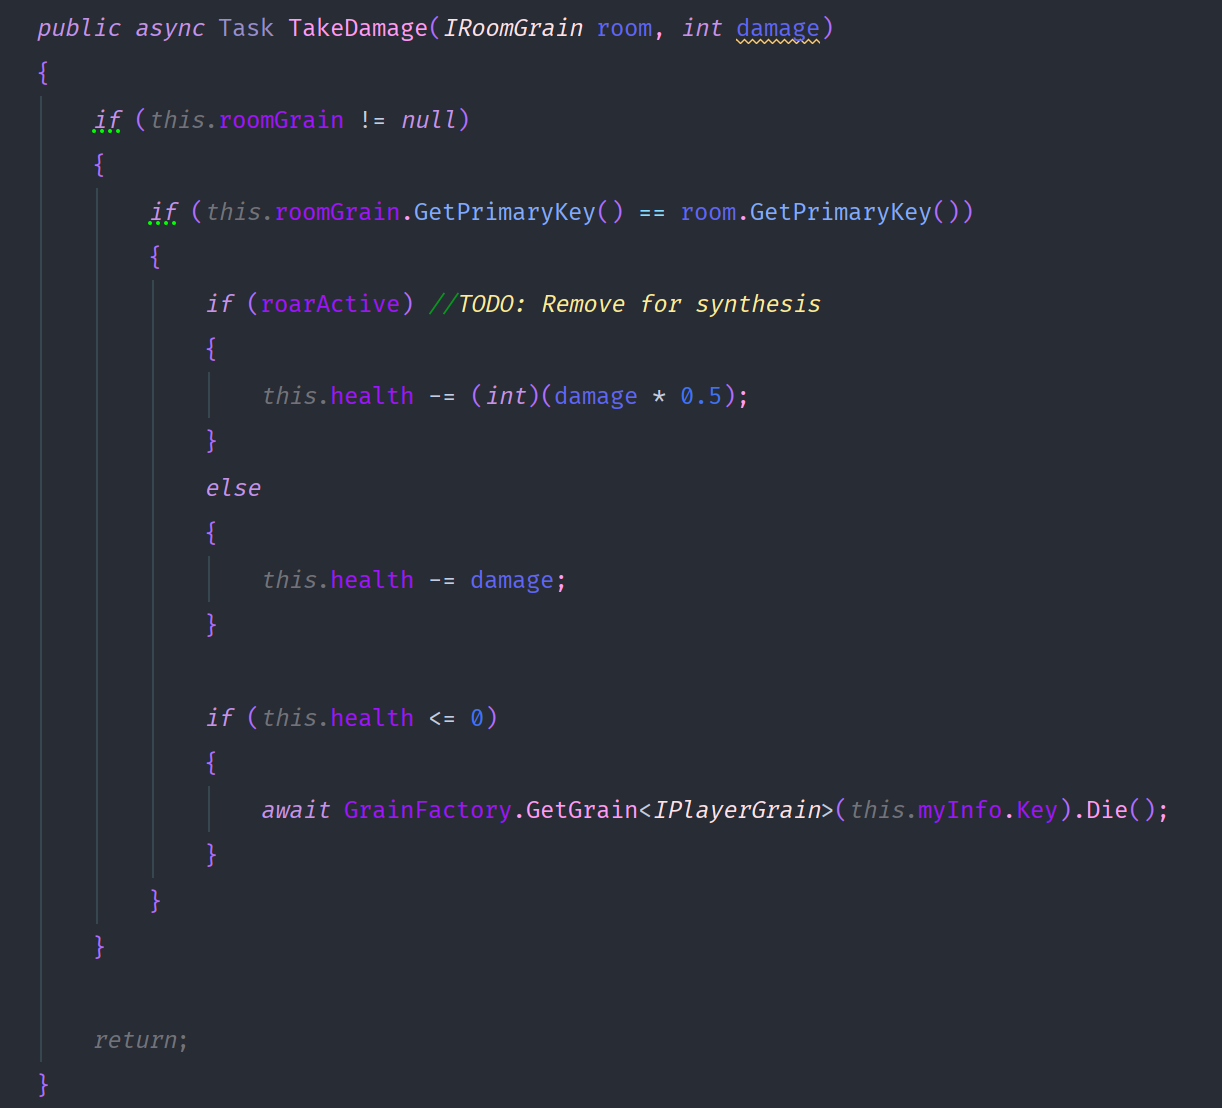
\includegraphics[width=0.8\linewidth]{Materials/Decomposition/TakeDamage}
	\caption{The player's TakeDamage method. Note the if case for when the roar ability is active. Having this if statement means we either need more combinators to describe the synthesis we want, or we have to accept we have dead code. }
	\label{PlayerTakeDamage}
\end{figure}
One can now ask, why is it important not to have dead code? Having dead code means we have fragments of other variations in the code. This means we suddenly have code that does not necessarily makes sense in the current context. A consequence of this could be that we try to access an object that does not exist, making the whole program crash. In general we risk unexpected behaviour which in worst case leads to a crash. This can however be mitigated through thorough testing, showing that it is at least not immediately apparent how the code will show unexpected behaviour based on the dead code \todo{Do we agree that's how testing works?}.\\
On the concrete example of \textit{'TakeDamage'} we see that \textit{'roarActive'} has to be true for the player to take half damage. Designing the player such that the only time this field is set to true is in the roar ability, it would be rather safe to leave the if statement in, as it should not ever be reachable this way. This also made the argument for choosing to leave the dead code and simplify modularization of abilities. However, as we ran out of development time we have not been able to refactor the old code. It could however easily be refactored such that we used dependency injection to give the player an ability which would be its own object with a \textit{'useAbility'} method allowing the player object to call this whenever it needs. The fireball implementation would then call the enemy's \textit{'kill'} method with a high damage value, and the roar implementation would set \textit{'roarActive'} in the player.\\ \todo{Stating we are not going to change player implementation.}
One could argue that in traditional software development it would not be possible to leave dead code in the implementation as we argue in the above that we can, and thus the above is not truly a modularization of the player. To that it could be argued that creating the combinators using the semantic type \textit{'damageTaken} opens up for possible extensions. If there had to be made combinators for how the player takes damage, we have effectively unified what caused the original problem, that an ability both could deal damage and affect how the player takes damage. The only problem here is how we carry this information and rather poor scaleability. Before getting into that we will summarize on the semantics that makes a player.\\
In our concrete implementation the semantics of a player is split in three parts, its actions, its ability and how it takes damage. As already discussed, we have the switch case of actions a player can take and to be able to perform an ability a case needs to be added here. Semantically we can call this a \textit{'case'}. Not surprisingly we can relate the players ability to the semantic type \textit{'ability'}. Lastly we will refer to how the player takes damage with the semantic type \textit{'damageTaken'}. We can thus describe a player as: \textit{string $\cap$ case, string $\cap$ ability, string $\cap$ damageTaken $\to$ MyResult $\cap$ player}. \todo{Unsure if this is a way to long explanation just to reach this rather anticlimactic point?}

\begin{figure}[H]
	\centering
	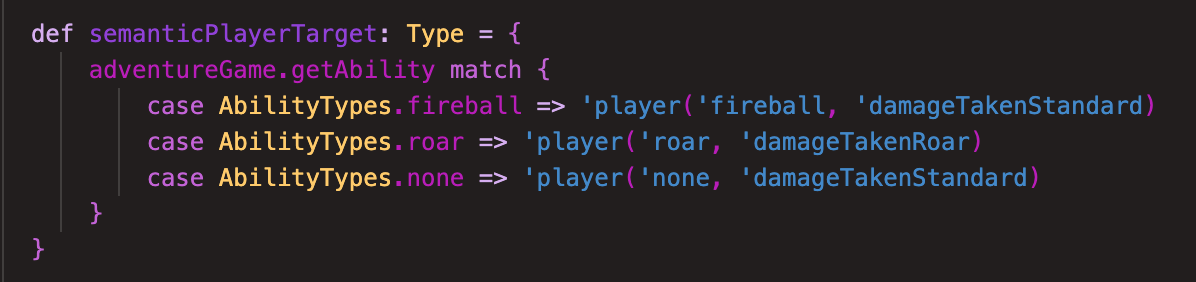
\includegraphics[width=0.9\linewidth]{Materials/Decomposition/SemanticTargetPlayer}
	\caption{The function determining what semantic types in the player we are looking for in our variations.}
	\label{SemanticTargetPlayer}
\end{figure}
So why did we say this approach would scale poorly? This is due to how we carry the information about which variation we want to synthesize. To this we are using \textit{kinding} which allows us to specific about our semantic types. As seen in \autoref{SemanticTargetPlayer} we can for instance have a semantic type \textit{'player('fireball, 'standardDamageTaken}. Here the types \textit{fireball} and \textit{damageTakenStandard} are kindings of respectively \textit{ability} and \textit{damageTaken}. The semantic types (of the same names) can now take these kindings and that way we create the variation we want. For the player the semantic type \textit{'case'} takes the same kinding as the semantic type \textit{'ability'} and that way we always get the corresponding ability to a case. But as we already have noted a player takes two kindings. This is the reason this approach does not scale. If we for each ability have to create combinators and create kindings to carry information forward it will not be feasible to write out all the possible outcomes when appending to the \textit{'semanticPlayerTarget'} function (seen in \autoref{SemanticTargetPlayer}).\\
We previously discussed how we could avoid using the semantic type \textit{'damageTaken'} and obtain more modularization by accepting dead code. Using this approach we can describe a player as: \textit{string $\cap$ case, string $\cap$ ability $\to$ MyResult $\cap$ player}. This approach would avoid introducing more kindings than \textit{ability} and would thus seem more scaleable. However, tweaking the damage reduction for the player would seem problematic but adding other ways to deal damage and adding abilities with different 'purpose' than dealing damage and reducing it would also seem easily done.\\

The player fulfilled the purpose of being an entity with timers. When synthesising the abilities we also include code for timers for the two possible abilities. We can thus say that we successfully can synthesize actor code which uses timers. However, these timers are very simple. They do not require disposing as the player only seizes to exist when the program is closed. Further, these timers are never recurring, so they only fire when the player asks them to. This essentially means that our only consideration with timers for the player is the abilities cool downs (the time before we can use the ability again, because being able to use the abilities repeatedly would make the player way too strong).  